\section{集成电路}
\begin{figure}[htbp]
	\centering
	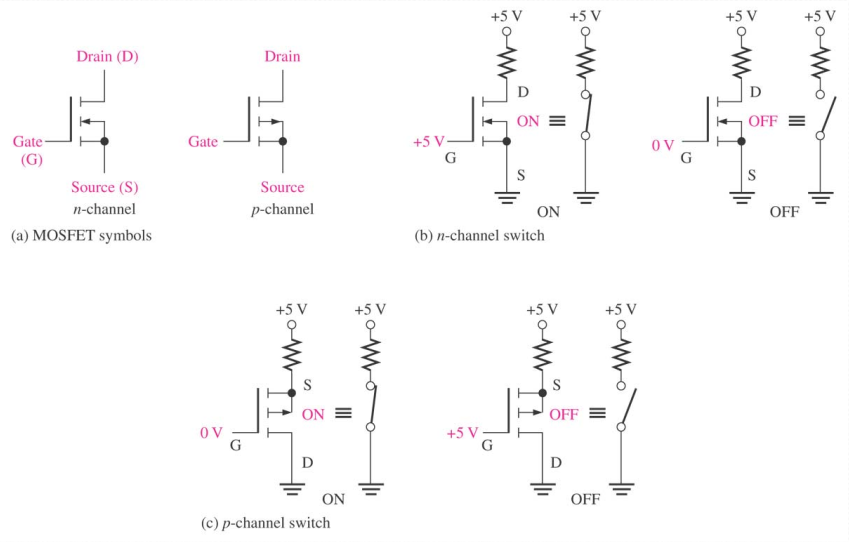
\includegraphics[width=0.8\linewidth]{fig/cmos.PNG}
	\caption{CMOS电路:\large\textbf{$n$内高,$p$外低}}
\end{figure}
\begin{figure}[htbp]
	\centering
	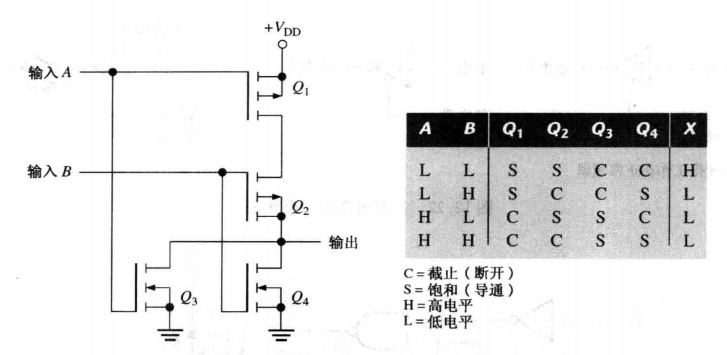
\includegraphics[width=0.6\linewidth]{fig/cmos_ex.PNG}
	\caption{CMOS或非门}
\end{figure}
\begin{figure}[htbp]
	\centering
	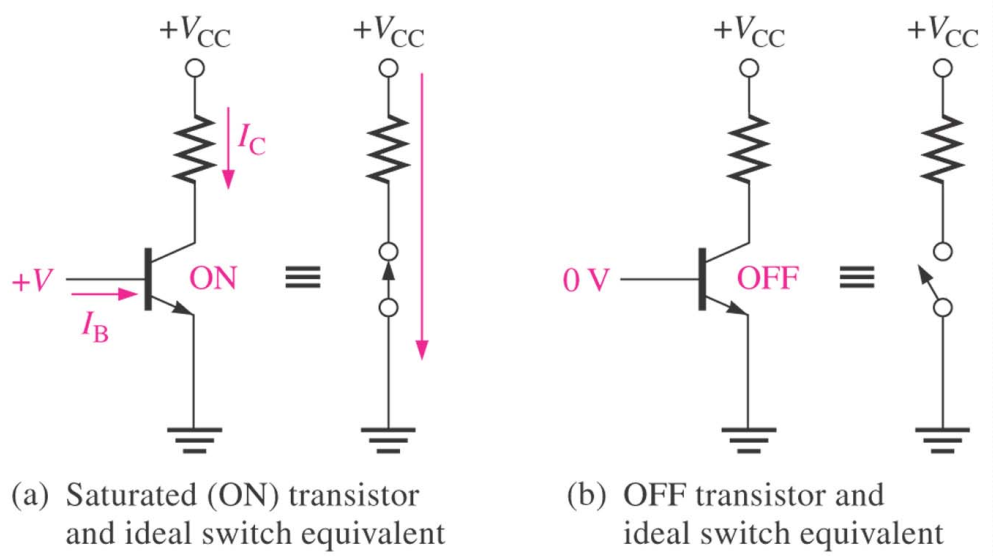
\includegraphics[width=0.6\linewidth]{fig/ttl.PNG}
	\caption{TTL电路}
\end{figure}
\begin{figure}[htbp]
\label{ttl_inverse}
	\centering
	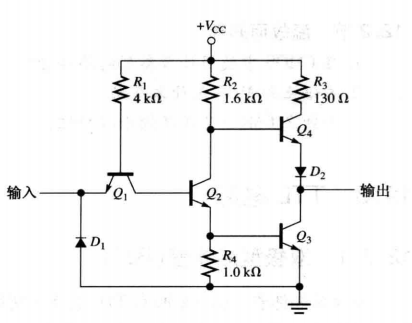
\includegraphics[width=0.6\linewidth]{fig/ttl_ex.PNG}
	\caption{TTL反相器}
\end{figure}
\par 由图\ref{ttl_inverse},$Q_1$被$V_{CC}$上拉,始终导通. 若输入为高电平,$Q_2$导通,$Q_3$导通,输出被下拉为低电平. 同时,$Q_2$在集电极处足够低的电压可以使$Q_4$截至.
\begin{figure}[htbp]
	\centering
	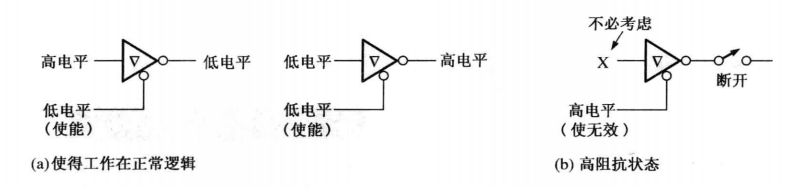
\includegraphics[width=0.6\linewidth]{fig/three_gates.PNG}
	\caption{三态门}
\end{figure}